\def\year{2017}\relax
%File: formatting-instruction.tex
\documentclass[letterpaper]{article}
%\usepackage{aaai17}
\usepackage{times}
\usepackage{helvet}
\usepackage{courier}
\frenchspacing
\setlength{\pdfpagewidth}{8.5in}
\setlength{\pdfpageheight}{11in}
\usepackage{cite}
\usepackage{subcaption}
\usepackage{hyperref}

\usepackage{graphicx}

\usepackage{titling}
\graphicspath{{figures/final/}}


\pdfinfo{
/Title (Supplementary Material: Shaping Model-Free Reinforcement Learning with Model-Based Pseudorewards)}
\setcounter{secnumdepth}{0}  
 \begin{document}
% The file aaai.sty is the style file for AAAI Press 
% proceedings, working notes, and technical reports.
%

\title{Supplementary Material: Shaping Model-Free Reinforcement Learning with Model-Based Pseudorewards}
%\subtitle{Shaping Model-Free Reinforcement Learning with Model-Based Pseudorewards}
\date{}
\maketitle

\pagebreak

\section{Omniscient Dyna (maze task, mountain car to come; figure captions to come)}

\begin{figure}[ht]
\centering
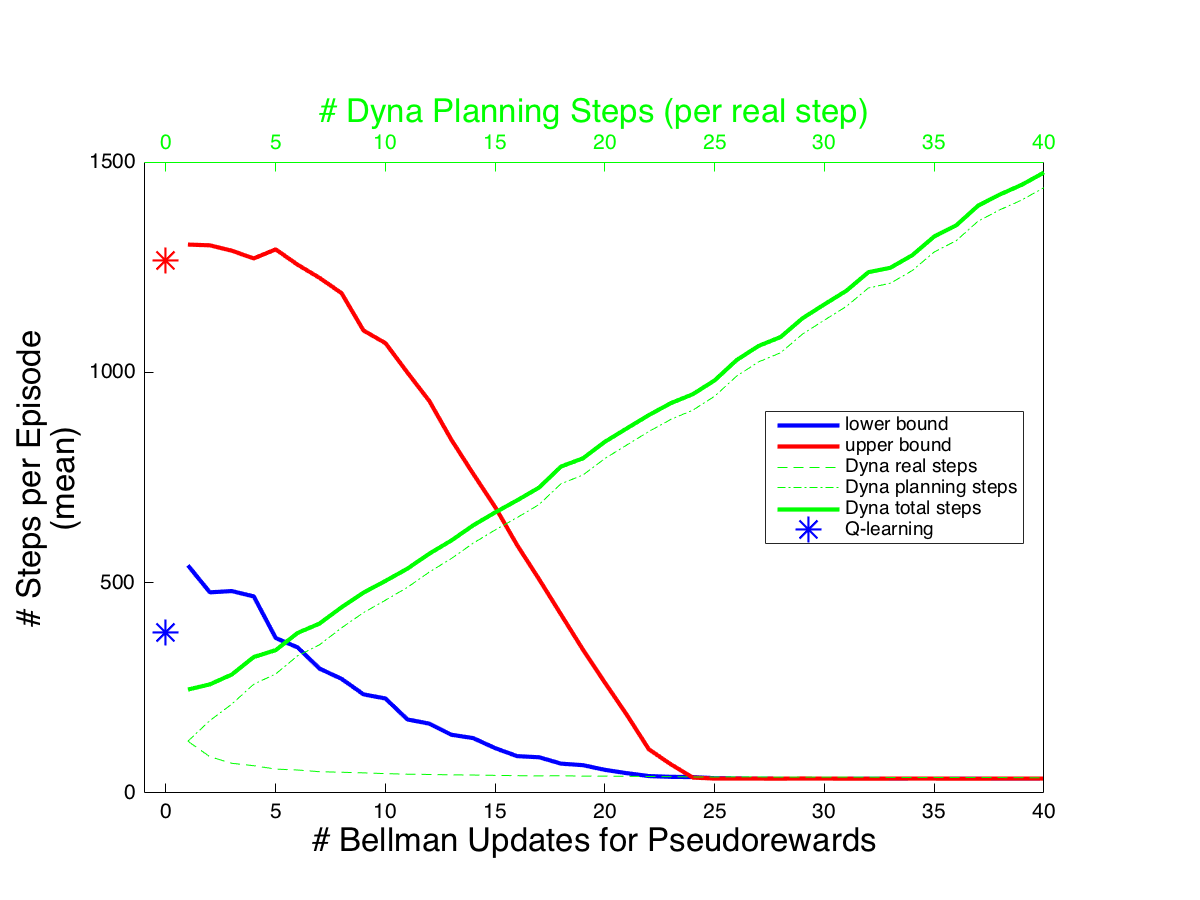
\includegraphics[width=0.5\textwidth]{learning_vs_PRiterations_omniscientDYNA_mean}
\caption{omniscient Dyna}
\label{fig:sS1a}
\end{figure}

\begin{figure}
\centering
\begin{subfigure}{.4\textwidth}
  \centering
  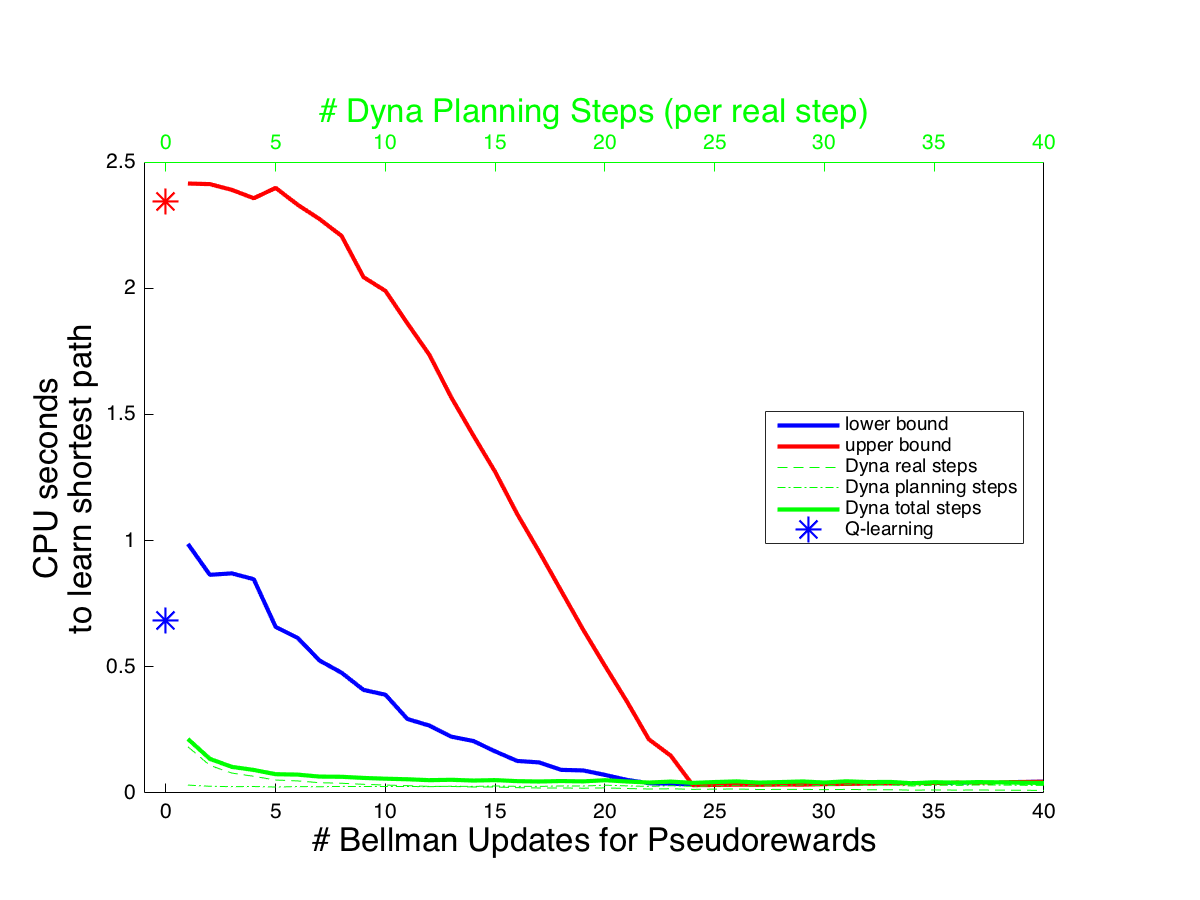
\includegraphics[width=.95\linewidth]{cpus_vs_PRiterations_omniscientDYNA_toGoal}
  \caption{CPU time}
\end{subfigure}
\begin{subfigure}{.4\textwidth}
  \centering
  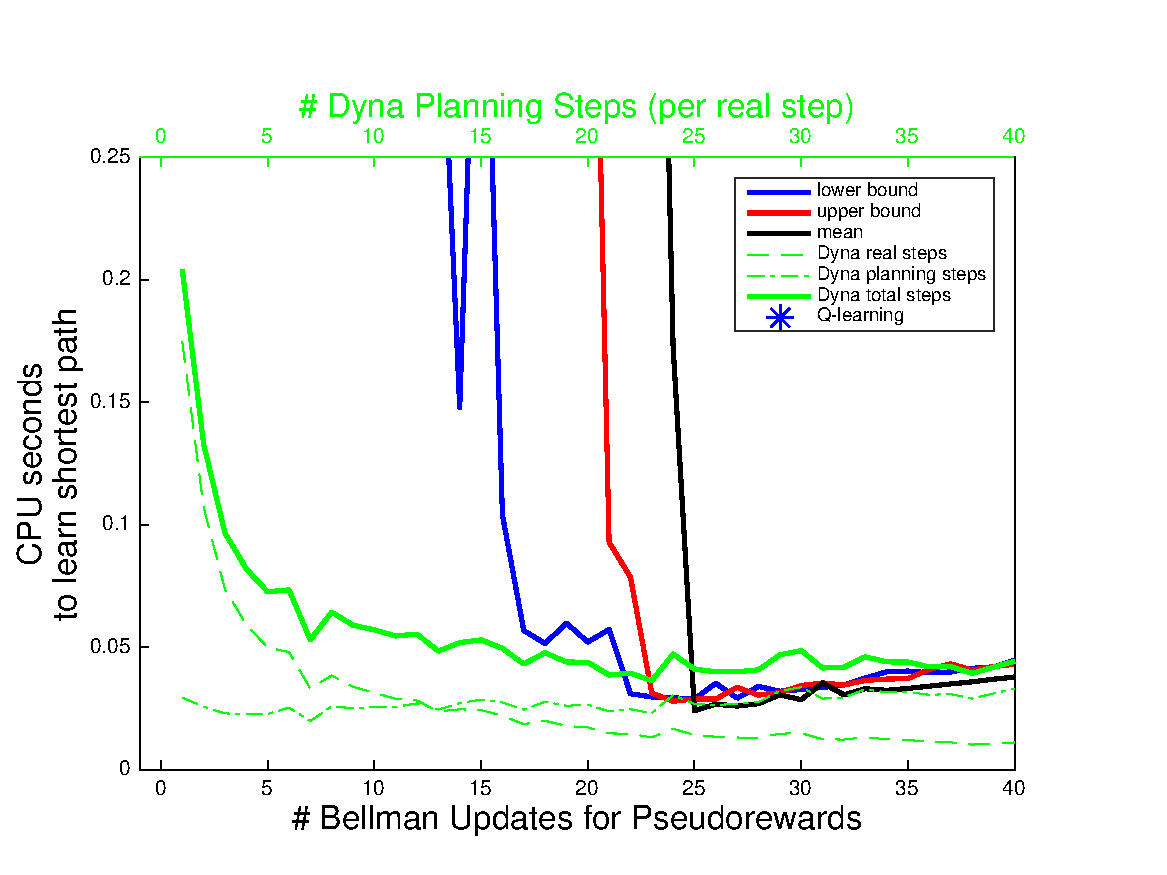
\includegraphics[width=.95\linewidth]{cpus_vs_PRiterations_omniscientDYNA_toGoal_closeup}
  \caption{close-up}
\end{subfigure}
\caption{omniscient Dyna}
\label{fig:S1b}
\end{figure}

\pagebreak

\section{Non-omniscient pseudoreward estimation (maze task, mountain car to come)}

\begin{figure}[ht]
\centering
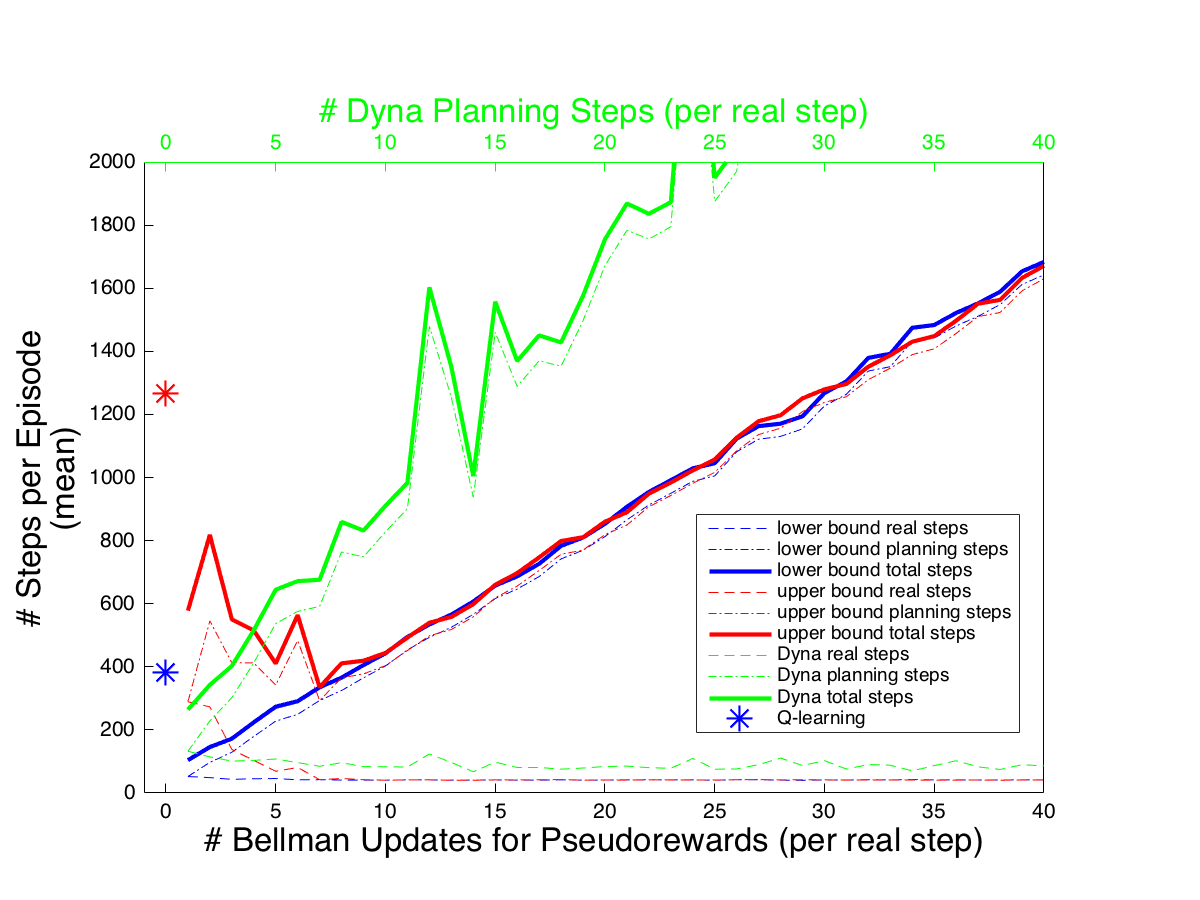
\includegraphics[width=0.5\textwidth]{learning_vs_PRiterationsLearnMod_DYNA_mean}
\caption{Non-omniscient pseudoreward estimation}
\label{fig:S2a}
\end{figure}

\begin{figure}
\centering
\begin{subfigure}{.4\textwidth}
  \centering
  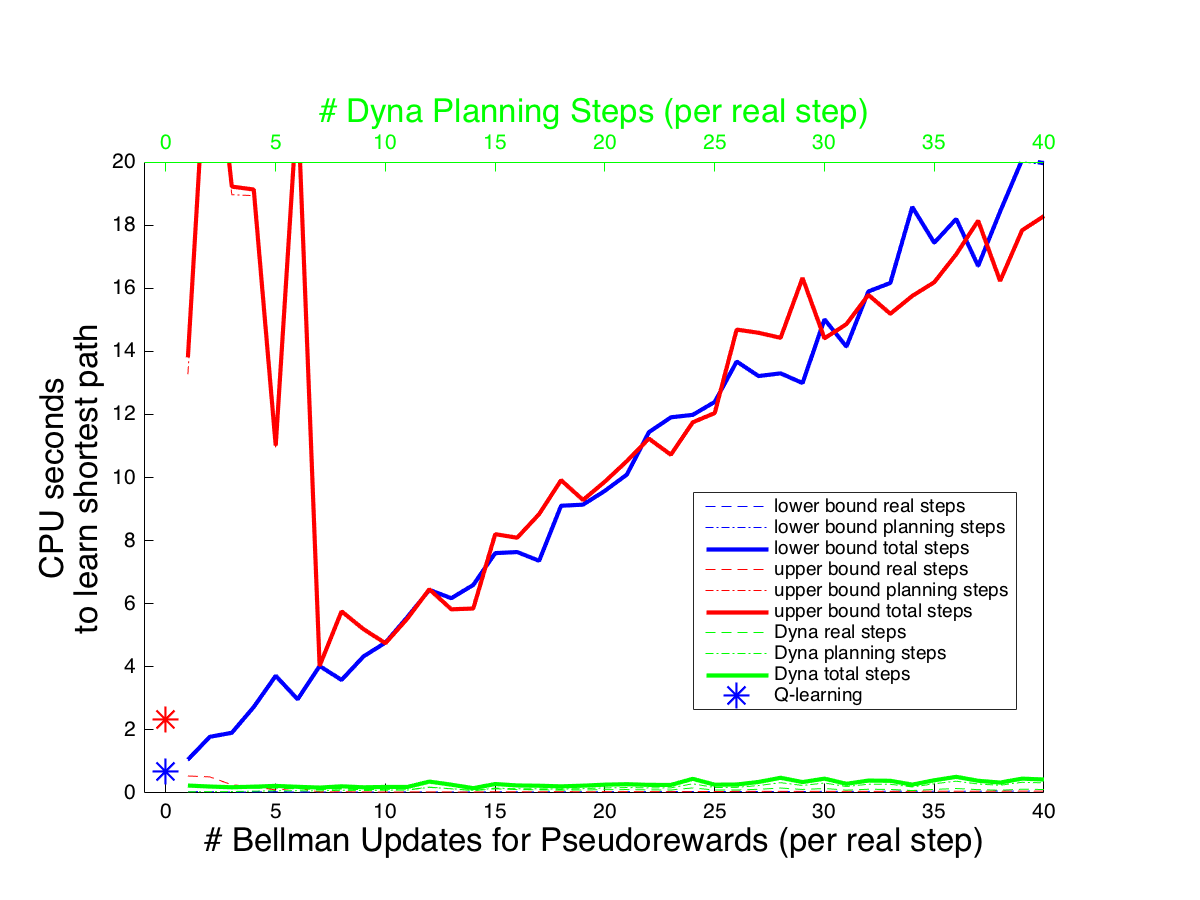
\includegraphics[width=.95\linewidth]{cpus_vs_PRiterationsLearnMod_DYNA_toGoal}
  \caption{CPU time}
\end{subfigure}
\begin{subfigure}{.4\textwidth}
  \centering
  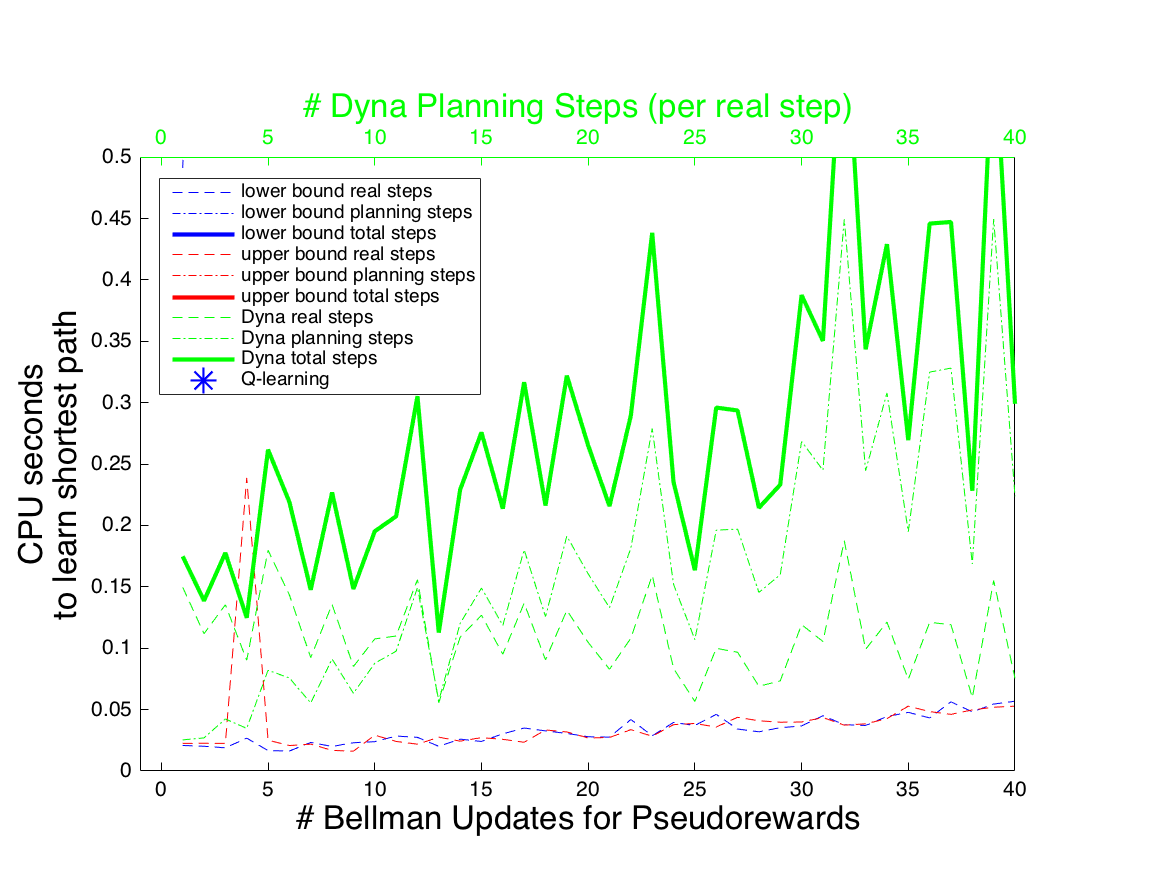
\includegraphics[width=.95\linewidth]{cpus_vs_PRiterationsLearnMod_DYNA_toGoal_closeup}
  \caption{close-up}
\end{subfigure}
\caption{Non-omniscient pseudoreward estimation}
\label{fig:S2b}
\end{figure}

\pagebreak

\section{Prioritized sweeping (maze task, mountain car to come)}

\begin{figure}[ht]
\centering
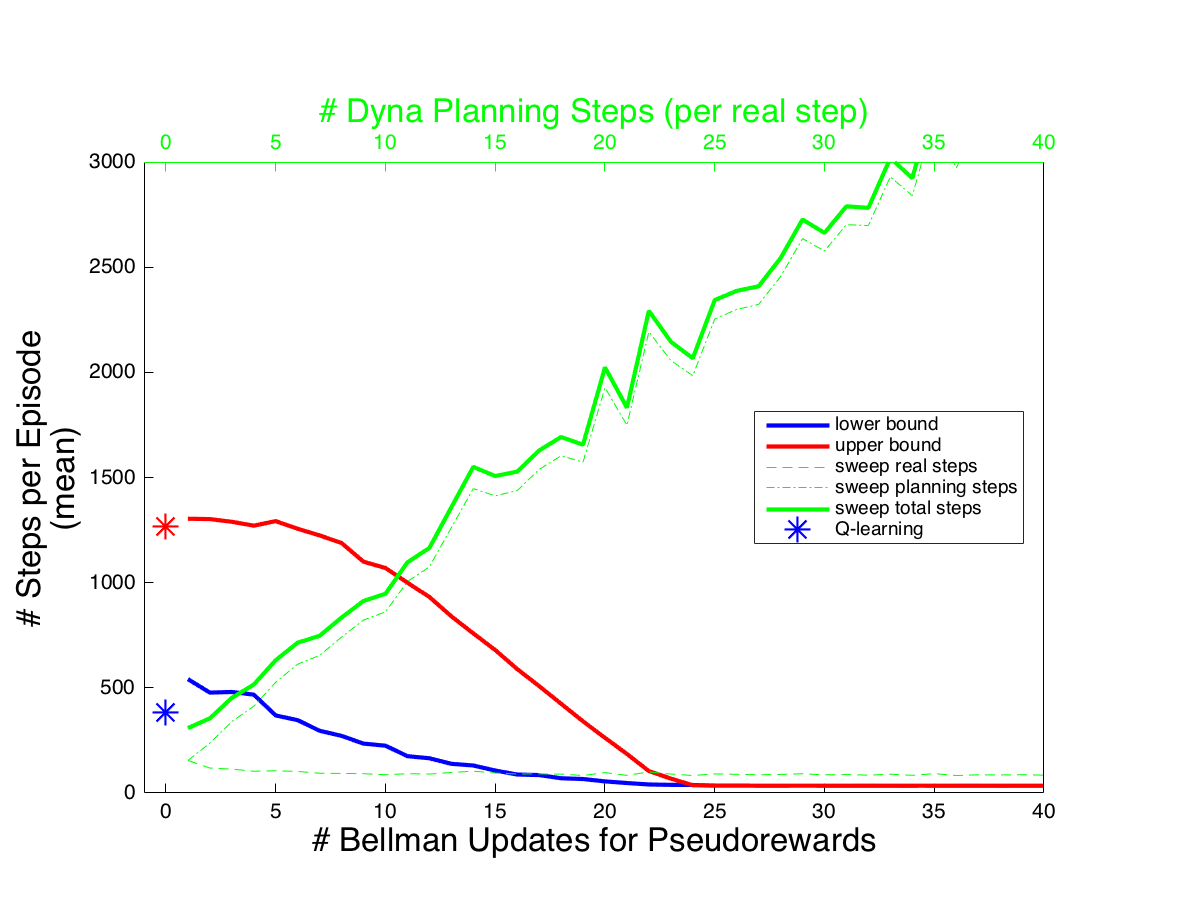
\includegraphics[width=0.5\textwidth]{learning_vs_PRiterationsSweeping_DYNA_mean}
\caption{Prioritized sweeping}
\label{fig:S3a}
\end{figure}

\begin{figure}[ht]
\centering
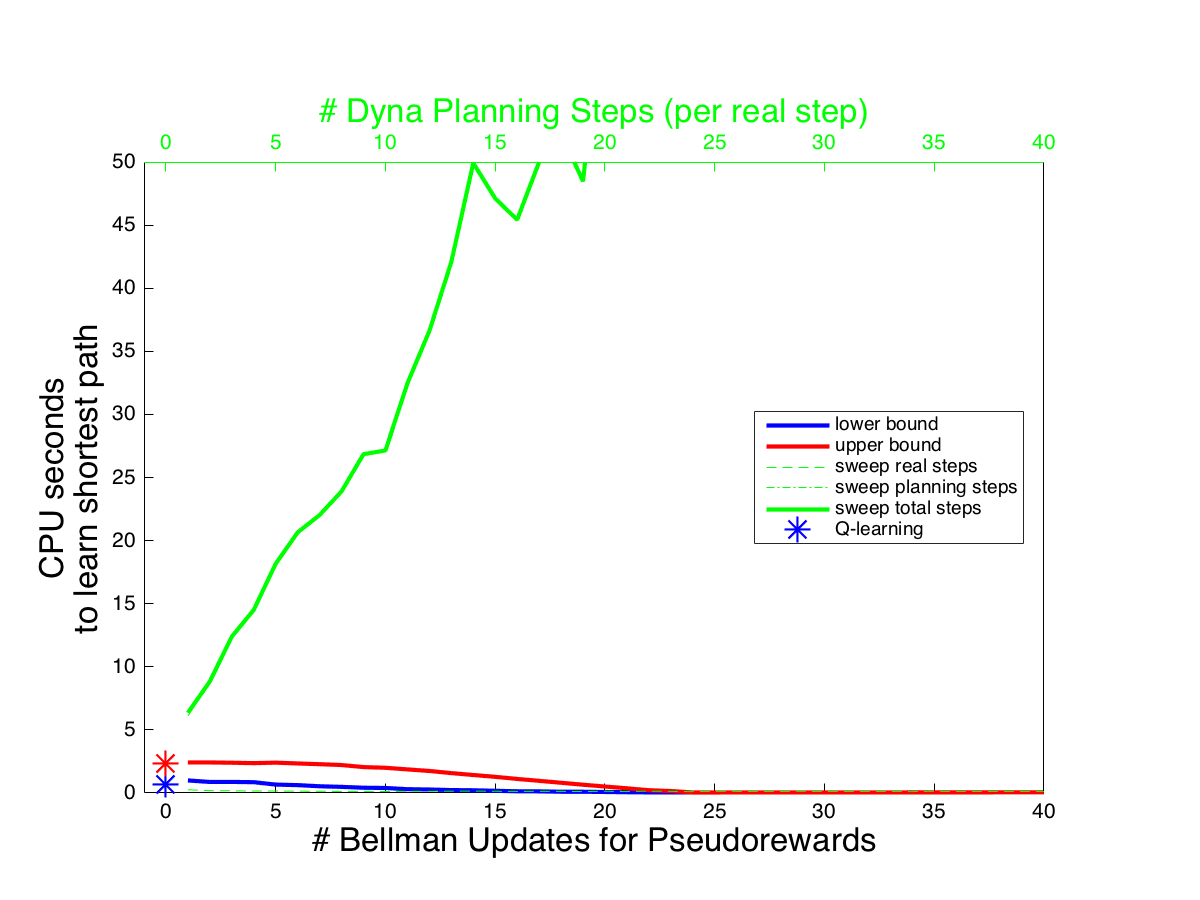
\includegraphics[width=0.5\textwidth]{cpus_vs_PRiterations_sweeping_toGoal}
\caption{CPU time}
\label{fig:S3b}
\end{figure}

\end{document}
